%\documentclass[10pt,handout]{beamer}
\documentclass[10pt]{beamer}
\usepackage[english]{babel} % Anpassa efter svenska. Ger svensk logga.
\usepackage[utf8]{inputenc} % Anpassa efter linux
\usepackage{graphicx}
\usepackage{../common/beamerthemeUppsala}
%\usetheme{Uppsala}
%\usecolortheme{UU} % Anpassa efter UU:s frger och logga
%\hypersetup{pdfpagemode=FullScreen} % Adobe Reader ska ppna fullskrm
\setbeamertemplate{itemize items}[circle]

% \usepackage{beamerthemesplit}
\usepackage{amsmath}
\usepackage{amssymb}
% \usepackage{graphics}
% \usepackage{graphicx}
% \usepackage{epsfig}
% \usepackage[latin1]{inputenc}
 \usepackage{color}
% \usepackage{fancybox}
% \usepackage{psfrag}
% \usepackage[english]{babel}
 \setbeamertemplate{footline}{\hfill\insertframenumber/\inserttotalframenumber}


% Read in commands
% Course settings
\newcommand{\currentsemester}{Autumn 2024}

% New commands
\newcommand{\bfm}[1]   {\mbox{\boldmath{${#1}$}}}
\newcommand{\Prob}   {\mbox{\textnormal{P}}}
\newcommand{\uured}[1]{\textcolor{uured}{#1}}

% Eqds
\def\eqd{\,{\buildrel d \over =}\,}

% Math operators
\DeclareMathOperator{\E}{\mathbb{E}}
\DeclareMathOperator{\V}{\mathbb{V}}


%%%%%%%%%%%%%%%%%%%%%%%%%%%%%%%%%%%%%%%%%%%%%%%%%%%%%%%%%%%%%%%%%%

\setlength{\parskip}{3mm}
\title[]{{\color{black}Machine learning -- Block 2}}
\author[]{M{\aa}ns Magnusson\\Department of Statistics, Uppsala University}
\date{November 2022}


\begin{document}

\frame{\titlepage
% \thispagestyle{empty}
}

%%%%%%%%%%%%%%%%%%%%%%%%%%%%%%%%%%%%%%%%%%%%%%%%%%%%%%%%%%%%%%%%%%


\begin{frame}{This week's lecture}
\begin{itemize}
\item Trees
\item Bagging
\item Random Forest
\item Boosting (Trees)
\end{itemize}
\end{frame}



%%%%%%%%%%%%%%%%%%%%%%%%%%%%%%%%%%%%%%%%%%%%%%%%%%%%%%%%%%%%%%%%%%

\frame{\frametitle{Assignment 1}

Short evaluation.

}

\section{Decision trees}
\frame{\frametitle{Decision trees: basic idea}
A popular method that can be used for both classification and regression is {\color{uured}decision trees}.\\[3mm]\pause
%We will discuss classification trees in this lecture - regression trees are analogous.\\[3mm]\pause
Have you ever played the game ''20 questions''?\\[3mm]\pause
Decision trees is more or less that game!\\[3mm]\pause
In the case of classification, the idea is to classify the new observation by asking a series of questions. Depending on what the answer to the first question is, different second questions are asked, and so on. Questions are asked until a conclusion is reached.
}

\frame{\frametitle{Decision trees: basic idea}
Consider the following data set with animal data:
{\small
\begin{table}[ht]
\begin{tabular}{l| l|l|l|l}
{\bf Name} & {\bf Body temp}& {\bf Gives birth}& {\bf Legs}& {\bf Class} \\
\hline
Human & warm-blooded & yes & yes & mammal\\
Whale & warm-blooded & yes & no & mammal\\
Cat & warm-blooded & yes & yes & mammal\\
Cow & warm-blooded & yes & yes & mammal\\\hline
Python & cold-blooded & no & no & reptile\\
Komodo dragon & cold-blooded & no & yes & reptile\\
Turtle & cold-blooded & no & yes & reptile\\\hline
Salmon & cold-blooded & no & no & fish\\
Eel & cold-blooded & no & no & fish\\\hline
Pigeon & warm-blooded & no & yes & bird\\
Penguin & warm-blooded & no & yes & bird
\end{tabular}
\end{table}}
}

\frame{\frametitle{Decision trees: basic idea}

\begin{enumerate}
\item Does it give live birth? \pause (mammal)
\item Is it warm-blooded? \pause (bird)
\item Does it have legs? \pause (reptile)
\item Else (fish)
\end{enumerate}

}


\frame{\frametitle{The regions of a tree}

\begin{figure}[h]
\centering
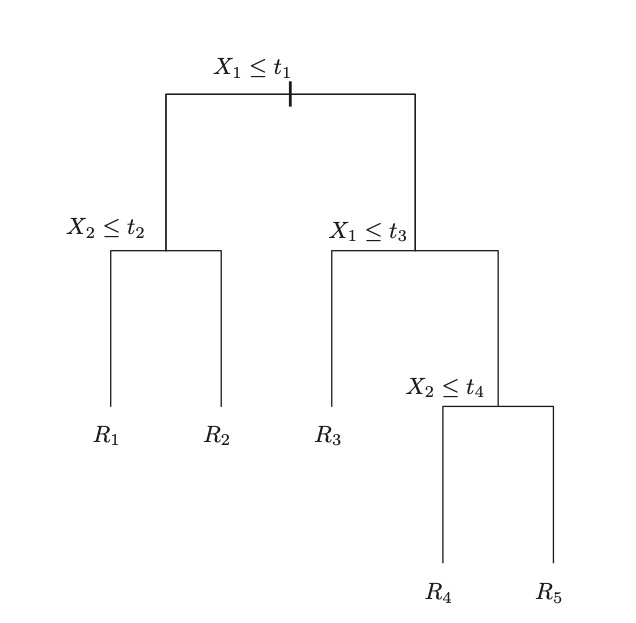
\includegraphics[width=0.45\textwidth]{fig/ISL_8_3_b.png}
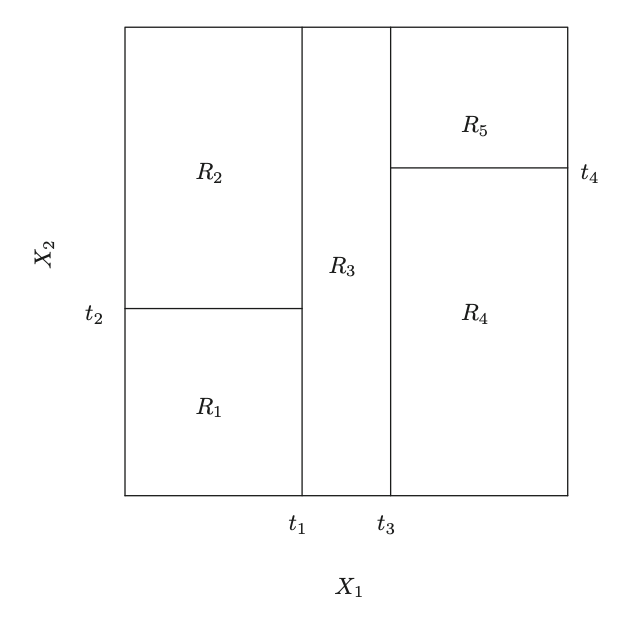
\includegraphics[width=0.45\textwidth]{fig/ISL_8_3_a.png}
\caption{Regions of a tree (Garreth et al, 2013, Fig. 8.3)}
\end{figure}

}



\frame{\frametitle{Regression Trees}

\[
T(x) = \sum^M_{m=1} \gamma_m I(x \in R_m)\,,
\]
where $M$ is the total number of regions and $I(x \in R_m)$ is an indicator variable if $x_i$ belongs to region $R_m$. $\gamma_m$ is the prediction for region $m$.

}

\frame{\frametitle{Regression Trees}

\begin{figure}[h]
\centering
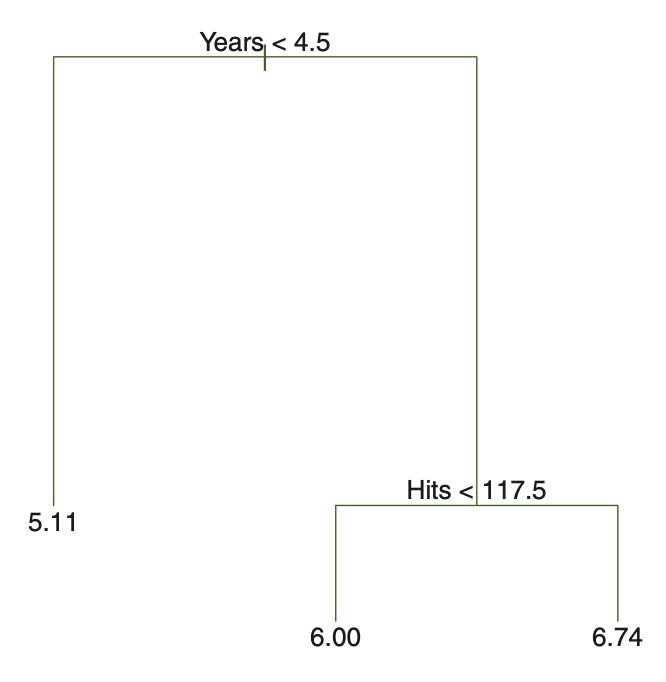
\includegraphics[width=0.5\textwidth]{fig/ISL_8_1_tree.png}
\caption{Regression Tree (Garreth et al, 2013, Fig. 8.1.)}
\end{figure}

\begin{itemize}
\item The \texttt{Hitters dataset}: Salaries of Baseball players.
\item The end of the tree contain the observations.
\end{itemize}
}



\frame{\frametitle{Regression Trees}

\begin{figure}[h]
\centering
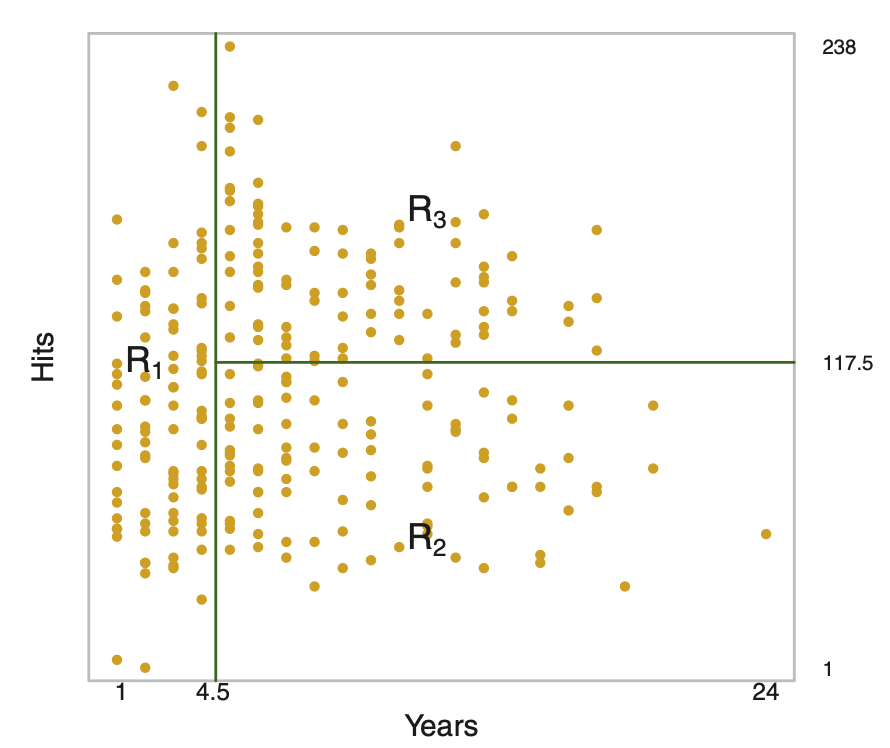
\includegraphics[width=0.8\textwidth]{fig/ISL_8_2_tree.png}
\caption{\texttt{Hitters} data and regression tree regions (Garreth et al, 2013, Fig. 8.2.)}
\end{figure}

}


\frame{\frametitle{Growing a Decision Tree}

\begin{enumerate}
\item A tree has two groups of parameters $\Theta = (\gamma, R)$ that we need to learn.\pause
\item We want a tree that minimize $L(\theta) = (y_i - T_\Theta(x_i))^2$\pause
\item Usually we estimate $\gamma_m$ as the mean of $y_i$ in the region as:
\[
\hat{\gamma}_m = \frac{1}{N_m} \sum_{x_i \in R_m}^{N_m} y_i\,,
\]
where $N_m$ is the number of observations in region $R_m$.\pause
\item Learning $R_m$ is generally computationally infeasable so we use a greedy heuristic.
\end{enumerate}

}



\frame{\frametitle{Growing a Decision Tree: Greedy Algorithm}


Let $\mathcal{S}$ be the set of all observations $\{1,...,N\}$ and \texttt{S[[m]]} be the set of observation indecies in $R_m$ and \texttt{l} is the minimal number of leafs per node.

Input: $\mathcal{S}, \texttt{X}, \texttt{y}, \texttt{l}$

\begin{enumerate}
\item \texttt{S[[1]]} = $\mathcal{S}$,\texttt{M = 1}, \texttt{m = 1}
\item \texttt{while m <= M} then do:
\begin{enumerate}
\item \texttt{if(size(S[[m]]) >= 2*l)}
\begin{enumerate}
\item \texttt{S[[M+1]]}, \texttt{S[[M+2]]}, \texttt{j[m]}, \texttt{s[m]} = \\ \texttt{split\_tree(X[S[[m]],], y[S[[m]],],l)}
\item \texttt{M = M + 2}
\end{enumerate}
\item \texttt{else}
\begin{enumerate}
\item compute $\hat{\gamma}$ for \texttt{S[[m]]}
\end{enumerate}
\item \texttt{m = m + 1}
\end{enumerate}
\end{enumerate}

Output: $\texttt{j}, \texttt{s}, \gamma$

Example:
\texttt{j = \{Years, Hits\}}, \texttt{s = \{4.5, 117.5\}}, $\hat{\gamma} = \{122, 317, 245\}$

}

\frame{\frametitle{How to do a split - the math.}

Here we try to compute Eq. (9.12-9.14) in ESL:

\[
R_1(j,s) = \{X|X_j\leq s \}\text{ and } R_2(j,s) = \{X|X_j > s \}
\]

\[
\min_{j,s} \left(\min_{c_1} \sum_{x_i \in R_1(j,s)} (y_i - c_1)^2 + \min_{c_2} \sum_{x_i \in R_2(j,s)} (y_i - c_2)^2\right)
\]

Inner minimization is solved by:
\[
\hat{c}_m = \frac{1}{N_m} \sum_{x_i \in R_m}^{N_m} y_i\,,
\]

}

\frame{\frametitle{How to do a split?}



Input: $\mathbf{X}, \mathbf{y}, l$

\begin{enumerate}
\item $SS$ = Inf \# Store sum of squares in matrix of dim $P\times N_s$
\item $S$ = Inf \# Store split point in matrix of dim $P\times N_s$
\item for $j \in \{1,...,P\}$ \# all features
\begin{enumerate}
\item for $k \in \{1,...,N_s\}$ \# all observations in set $s$
\begin{enumerate}
\item $s$ = $x_{k,j}$ \# Split point (use the value of x)
\item if ($|R_1(s, j)| < l$ or $|R_2(s, j)| < l$) next \# Dont create too few leaves
\item $\hat{c}_1$ = $\frac{1}{|R_1(s, j)|} \sum_{x_i \in R_1(s, j)} y_i$
\item $\hat{c}_2$ = $\frac{1}{|R_2(s, j)|} \sum_{x_i \in R_2(s, j)} y_i$
\item $SS_{k,j}$ = $\sum_{x_i \in R_1(s, j)} (y_i - c_1)^2 + \sum_{x_i \in R_2(s, j)} (y_i - c_2)^2$ \# Compute Sum of Squares
\item $S_{k,j}$ = s
\end{enumerate}
\end{enumerate}
\item $k_{final}, j_{final} = \min_{k,j} SS$
\item $s_{final} = S_{k_{final},j_{final}}$
\item return $R_1(s_{final}, j_{final}), R_2(s_{final}, j_{final}), s_{final}, j_{final}$
\end{enumerate}
}



\frame{\frametitle{Decision trees: Classification Trees}

How do we do if we have a classification tree?\pause

We just change the loss function.\pause

Let $p(j|t)$ be the fraction of observations in class $j$ at the node $t$ and let $c$ be the number of classes.\pause

The {\color{uured}Gini} for node $t$ is defined as
\[
Gini(t)=1-\sum_{j=1}^c(p(j|t))^2
\]\pause
Gini is a measure of ''impurity''. If all observations belong to the same class, then
\[
Gini(t)=1-1^2-0-\ldots-0=0.
\]\pause
The Gini is maximized when all classes have the same number of observations at $t$.\\[2mm]\pause
One criterion for splitting could be to minimize the Gini in the next level of the tree. That way we will get ''purer'' nodes.
}


%\frame{\frametitle{Decision trees: the best split}
%The situation becomes a bit more complicated if we take into account that the children can have different numbers of observations. \pause To account for this, we try to maximize the gain:
%\[
%Gain=Gini(t)-\sum_{j=1}^k \frac{n_{v_j}}{n_t}Gini(v_j)
%\]
%where $v_j$ are the children and $n_i$ are the number of observations at node $i$.\\[2mm]\pause
%This is equivalent to minimizing $\sum_{j=1}^k \frac{n_{v_j}}{n_t}Gini(v_j).$\\[2mm]\pause
%Sometimes other impurity measures than Gini are used. One example is the {\color{uured}entropy}:
%\[
%Entropy(t)=-\sum_{i=1}^cp(i|t)\log_2p(i|t).
%\]
%}

\frame{\frametitle{Important concepts}
\begin{itemize}
\item {\color{uured}Tree depth:} the length of the longest path from the root to a leaf (i.e. greatest number of questions that the tree can ask).\\[2mm]\pause
\item {\color{uured}Leaf size:} the number of observations in a leaf.\\[2mm]\pause
\end{itemize}
Decision trees can become quite large, which may lead to:
\begin{itemize}
\item Overfitting (high variance)
\item Difficulties interpreting the tree\\[2mm]\pause
\end{itemize}
The solution to this is
\begin{itemize}
\item {\color{uured}Pruning:} forcing the tree to be smaller by adding a {\color{uured}stopping condition}, e.g. a maximum depth or minimal leaf size.\pause
\item But decision trees are quite bad predition models...
\end{itemize}
}

%%%%%%%%%%%%%%%%%%%%%%%%%%%%%%%%%%%%%%%%%%%%%%%%%%%%%%%%%%%%%%%%%%

\section{Ensemble methods}

\frame{\frametitle{General idea of ensembles}
The idea of an ensemble is simple: If it difficult to find one really good model perhaps we can find several weaker models and combine their predictions.\\~\\
%
A simple example: Say you have one outcome $Y$ and 4 covariates $X_1,X_2,X_3,X_4$. The goal is to predict Y. A possible ensemble would be to fit
\begin{align*}
y=\alpha_1 + \beta_1X_1 + \epsilon_1\\
y=\alpha_2 + \beta_2X_2 + \epsilon_2\\
y=\alpha_3 + \beta_3X_3 + \epsilon_3\\
y=\alpha_4 + \beta_4X_4 + \epsilon_4
\end{align*}
and then use the mean of their predictions
\begin{equation}
\hat{y}_{ensemble}=\frac{1}{4}\sum_{i=1}^4 \hat{y}=\frac{1}{4}\sum_{i=1}^4(\hat{\alpha}_i + \hat{\beta}_iX_i)
\end{equation}

}

%
%
%

\frame{\frametitle{Two key parts of an ensemble}
\begin{itemize}
\item The prediction models (sometimes called `learners' in ML literature)
\begin{itemize}
\item A single model in an ensemble can be a simple or a complex model
\item Often the ensemble contains many simple models.
\item Wikipedia:``\textit{In statistics and machine learning, ensemble methods use multiple learning algorithms to obtain better predictive performance than could be obtained from any of the constituent learning algorithms alone}''
\end{itemize}
\item The weighting of each prediction in the final ensemble prediction
\begin{itemize}
\item Models/learners with better predictive power can be given larger weights in the final prediction
\item There are many complex algorithms for weighting together the predictions from many models
\end{itemize}
\end{itemize}
}


\frame{\frametitle{Ensambles of decision trees}
The most common type of ensembles is ensembles of decision trees.

We will focus on this case, but note that any type of model can be included in an ensemble in principle.\\~\\
}
%%%%%%%%%%%%%%%%%%%%%%%%%%%%%%%%%%%%%%%%%%%%%%%%%%%%%%%%%%%%%%%%%%



%\section{Bagging and Boosting}
\frame{\frametitle{Bagging and Boosting}

Remember, the error of a prediction/classification can be decomposed as
\begin{equation}
error = bias + variance + bayes error.
\end{equation}
\begin{itemize}
\item Complex models/strong learners (with many parameters) tend to have small bias and large variance (tend to be overfitted)
\item Shallow models/weak learners (with few parameters) tend to have small variance and large bias
\end{itemize}
\pause


\textbf{Bagging:} Ensemble methods that aim to decrease the variance of complex/strong learners with low bias and large variance\\~\\
\textbf{Boosting:} Ensemble methods that aim to decrease the bias of shallow/weak learners with low variance and large bias

%That is: Either choose models with small bias and reduce the variance with bagging, or choose models with small variance and reduce bias with boosting
}


\section{Bagging}

\frame{\frametitle{Bagging (Bootstrap AGGregating) -- Bootstrap improvement of prediction models}
Consider a sample of $N$ units.\\~\\
\textbf{Bagging algorithm:}
\begin{enumerate}
\item Draw, \textit{with replacement}, a random sample of $N$ units from the original sample
\item Fit a prediction model (e.g., a decision tree)
\item Repeat steps 1-2 $B$ times
\item Weight together the predictions from the B models into a final ensemble prediction
\end{enumerate}

\pause
Train several deep trees and combine their results by weighting together their predictions
}







%%%%%%%%%%%%%%%%%%%%%%%%%%%%%%%%%%%%%%%%%%%%%%%%%%%%%%%%%%%%%%%%%%

\subsection{Random forests}

\frame{\frametitle{Random Forest}

A random forest is a bagging ensemble method, but with one extra step. Consider a sample of N units and K observed covariates/features\\~\\

Random forest algorithm:
\begin{enumerate}
\item Draw, \textit{with replacement}, a random sample of $N$ units from the original sample
\item \textbf{Draw,  \textit{without replacement}, a random subset of $k$ covariates/features}
\item Fit a prediction model (e.g., a decision tree)
\item Repeat step 1-3 $B$ times
\item Weight together the predictions from the B models into a final ensemble prediction
\end{enumerate}

It is common to use $k=\sqrt{K}$ (rounded down) for classification and $k=K/3$ for regression. But these are only rules of thumb: $k$ is a \textit{tuning parameter}.
}

\frame{\frametitle{Random Forest, variance reduction}
	Consider each tree to be an i.i.d. random variable with variance $\sigma^2$.\\
	The average of these trees then have variance $\frac{1}{B}\sigma^2$. Trees constructed from the same set of covariates will be correlated and therefore not independent. The variance of the average of these correlated trees then becomes
	\begin{align*}
	\rho\sigma^2+\dfrac{1-\rho}{B}\sigma^2.
	\end{align*}
	The second term will vanish with increasing $B$ leaving just the first term left which is a function of the correlation between the trees and the variance. The remaining part of the variance is minimized by only consider a subset of the covariates when constructing trees - reducing the correlation between them.
}


\frame{
\frametitle{Differences between bagging and random forest:}
\begin{itemize}
\item In bagging, the trees are often highly correlated
\begin{itemize}
\item If some covariates are strong predictors of the outcome (in the training data), many trees in the `bag' will us the same covariates in their decisions
\end{itemize}
\item In a random forest, the trees are less similar/correlated since all covariates are not available when each tree is constructed.
\end{itemize}
This means that a random forest (with many trees) uses the predictive ability of all covariates rather than just a few, which usually improves out of sample performance.

}




%%%%%%%%%%%%%%%%%%%%%%%%%%%%%%%%%%%%%%%%%%%%%%%%%%%%%%%%%%%%%%%%%%

\section{Boosting}

\frame{\frametitle{Boosting}
In boosting, models are trained sequentially where each new model tries to target weak spots of the previous models in the ensemble to improve the performance of the ensemble

Boosting
\begin{enumerate}

\item Fit a prediction model/classifier (e.g., a decision tree) using the original sample
\begin{itemize}
\item Give the misclassified observations higher weights
\end{itemize}
\item Draw, \textit{with replacement},\textit{with probability proportional to the weights}, a random sample of $N$ units from the original sample
\item Fit a prediction model/classifier (e.g., a \emph{shallow} decision tree) using the new sample
\item Update the weights of each observation according to the average misclassification of the trained classifiers
\item Repeat step 2-4 B times
\item Weight together the predictions from the B models into a final ensemble prediction, giving larger weights to classifiers with smaller errors
\end{enumerate}

}

\frame{\frametitle{Boosting}
For boosting to work well, the updates of the weights must be chosen in some clever way. One successful method is \textit{gradient descent}.\\~\\

We will not focus more on the particular algorithms. For now, we are satisfied with understanding the concept of boosting:\\~\\
Train a bunch of classifiers sequentially. Force each new classifier to train more on data that the previous classifiers had problems with classifying by giving those samples a higher probability to be sampled.\\~\\

}


\frame{\frametitle{XGBoost}

\begin{enumerate}

\item State of the Art method\pause
\item Use gradient boosting trees with regularization\pause
\item Is scalable to very large data
\end{enumerate}

}



\end{document}
